\documentclass{sig-alternate-05-2015}

\usepackage{amsmath}
\usepackage{amssymb}

\begin{document}
%\doi{}
%\isbn{123-4567-24-567/08/06}
\title{Topic Models and Word Embeddings}
\subtitle{Master Thesis Expos\'e}

\numberofauthors{1}
\author{
\alignauthor
Stefan Bunk\\
       \affaddr{Hasso Plattner Institute, University of Potsdam}\\
       \affaddr{Prof.-Dr.-Helmert-Str. 2-3}\\
       \affaddr{14482 Potsdam, Germany}\\
       \email{stefan.bunk@student.hpi.uni-potsdam.de}
}
\date{9 June 2016}

\maketitle
\begin{abstract}
% Recently, distributed representations of words, called word embeddings, have gained traction for tasks such as .
% The master thesis will investigate
TODO
\end{abstract}

\section{Introduction}
A core task in natural language processing (NLP) is to understand the meaning of words.
Many downstream NLP tasks profit from this, for example text categorization, part-of-speech tagging, and machine translation.
A popular concept to qualify the meaning of a word is to look at the contexts, in which the word appears.
A famous quote by Firth says: ``You shall know a word by the company it keeps''~\cite{Firth1957}.
This assumption is also known as the distributional hypothesis.

Two existing approaches in this area are topic modelling and word embeddings.
Topic modelling assumes, that an author has certain topics in mind when writing a document, which are chosen beforehand.
For example, an author could decide to write a document about \emph{politics} (70~\%) in \emph{sports} (30~\%) and then picks the words ``coalition'', ``election'' and ``corruption'' for \emph{politics} and the words ``soccer'' and ``ball'' for \emph{sports}.
Topic modelling techniques, with Latent Dirichlet Allocation being the most popular one, try to recover the hidden topics in large corpora, i.e.\ find out that ``soccer'' and ``ball'' come from the same topic.
As topic models are probabilistic models and hence provide probability distributions as the result, the topics can be easily interpreted by humans.

In word embedding, each word is assigned a vector in a high-dimensional vector space.
These vectors are automatically learned using trained neural networks.
During the supervised training, each word must try to predict its surrounding words.
This way, the context of a word is encoded in the vector representation of a word.
Using a clever network architecture, these vectors exhibit interesting properties.
First, similar words tend to be in similar positions in the vector space.
For example, when looking for the most similar words for ``France'' using cosine distance, the model outputs ``Spain'', ``Belgium'', ``Netherlands'' and ``Italy''.
Second, the word vectors exhibit interesting linear relationships.
For example, when calculating the vector $vector("King") - vector("Man") + vector("Woman")$ and looking for the closest word at the vector result, the result is the word ``queen''~\cite{Mikolov2013b}.

The two approaches have different origins.
Word embeddings have their roots in the neural network and deep learning community, while topic modelling stems from Bayesian statistics.
Hence, there is relatively little research in combination of these two methods.
In this master thesis, we aim to explore potential synergies between these technologies.
In particular, it might be useful to investigate ``whether the the two types of models are complementary in the errors they make, in which case combined models could be an interesting avenue for future work''~\cite{Baroni2014}.

This expos\'e is organized as follows: Section~\ref{sec:related-work} will introduce topic modelling and word embeddings.
Section~\ref{sec:approach} will highlight potential for combining the two approaches.
Section~\ref{sec:data-sets-and-evaluation} will show different data sets and evaluation tasks to evaluate a joint system.

\section{Related Work}
\label{sec:related-work}
\subsection{Topic Modelling}

Many methods for modelling natural language text have been proposed.
An early popular method was tf-idf~\cite{SparckJones1972} scheme, which reduced each document in a corpus to a vector of term frequencies normalized by inverse document frequencies.
Later, Latent Semantic Analysis (LSA)~\cite{Deerwester1990} was proposed to reduce the large matrix to a smaller subspace using singular value decomposition.
While these approaches have their origins in linear algebra, topic models have been developed from a probabilistic view to allow better interpretation.
Topic models are generative probabilistic models of a document collection, which assume hidden topics have guided the generation of the text.
In this way of thinking, an author picks certain topics to write about, and then picks words associated with these topics for a concrete document.
The goal is then to uncover the unseen, so called ``latent'', topics from a text corpus.
All of these approaches have in common, that they assume a bag-of-words representation of documents.

\subsubsection{Earlier approaches}
A basic generative topic model is the mixture of unigrams model~\cite{Nigam2000}.
In this model, a topic is a fixed probability distribution over the vocabulary.
However, only one topic is allowed per document, which limits its predictive power.

A more sophisticated topic model is the probabilistic latent semantic analysis (pLSA), which allows multiple topics per document.
The model is fitted with an Expection-Maximization algorithm.
However, pLSA does not provide a full generative model applicable to unseen documents.
Also, as the number of parameters grows linearly with the number of training documents, it tends to overfit~\cite{Blei2003}.

\subsubsection{Latent Dirichlet Allocation (LDA)}
LDA was proposed by Blei et al.~\cite{Blei2003} for modelling text corpora and other collections of discrete data.
In an unsupervised fashion, it can automatically detect similarities between words and group them in one topic.
The number $K$ of topics is constant and must be chosen beforehand.
% TODO thesis: Add nice example document with figure, e.g. k=3 and some topics

LDA defines a topic as a distribution over a fixed vocabulary.
Different topics assign different probabilities to the same word, for example the word ``soccer'' would have a much higher probability in a \emph{sports} topic than in a \emph{politics} topics.
The opposite would hold for the word ``coalition''.
Note that a topic is only a distribution over words, i.e.\ LDA does not generate a name or a summary for a topic.

A document is assumed to consist of one or several topics with a certain, fixed distribution.
A document could be $20~\%$ about \emph{sports} and $80~\%$ percents about \emph{politics}, or $30~\%$ about \emph{climate}, $25~\%$ about \emph{cars} and $45~\%$ about \emph{politics}.
In general, LDA aims to generate sparse distributions for both cases, i.e.\ a topic should have only a few words (relative to the vocabulary of the entire corpus) with high probability and a document should have only a few topics.
This is governed by two scalar hyperparameters $\alpha$ and $\beta$, which influence two symmetrical prior Dirichlet distributions.

With these two hyperparameters, the generative document creation process of LDA can be summarized as follows:
\begin{enumerate}
       \item Fix number of topics $K$ in the document collection
       \item Choose word distributions $\phi_j \sim Dirichlet(\beta)$ for each topic $j \in \{1~..~K\}$
       \item Now, for each document $d$:
       \begin{enumerate}
              \item Choose topic distribution $\theta_d \sim Dirichlet(\alpha)$
              \item For each position $i$ in the document
              \begin{enumerate}
                     \item Choose topic $z_{d,i} \sim Multinomial(\theta_d)$
                     \item Choose word $w \sim Multinomial(\phi_{z_{d,i}})$ for current word
              \end{enumerate}
       \end{enumerate}
\end{enumerate}
This process is also illustrated in the probabilistic graphical model in Figure \ref{fig:lda}.
This model can also be seen as a soft-classification of documents: instead of assuming exactly one topic per document, each word in a document can potentially come from a different topic.

\begin{figure}
       \centering
       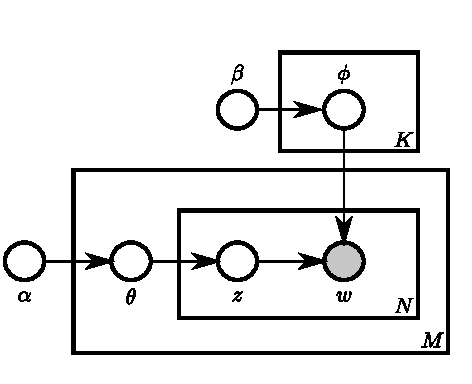
\includegraphics{figures/lda.pdf}
       \caption{Graphical model for Latent Dirichlet Allocation with $K$ topics, $M$ documents and $N$ words in a document.}
       \label{fig:lda}
\end{figure}

In reality, we only observe the words in the documents, and need to reverse engineer the hidden, ``latent'' parameters of the model, namely the word distribution per topic $\phi$, the topic distribution per document $\theta$ and the word-topic assignments $z$.
In this process, called \emph{inference}, we try to find the most probable parameter assignments, which could have generated our document collection.
Computationally, this is equivalent to finding the posterior distribution of the parameters given the observed words.
Blei et al.~\cite{Blei2003} propose an algorithm based on variational approximation, however Griffiths and Steyvers~\cite{Griffiths2004} proposed an algorithm based on Gibbs sampling.
% expand here: limiting distribution, sampling formula etc.

The output of running LDA on a corpus is three-fold:
\begin{itemize}
       \item Topics as set of similar words, e.g.\ the terms ``soccer'', ``ball'', ``league'' could form a topic named \emph{sports}.
       \item Topic distribution of a single word, e.g.\ the term ``jaguar'' occurs 80~\% in the \emph{cars} topic and 20~\% in the \emph{animals} topic
       \item Topic distribution inside a concrete document or inside the entire corpus
\end{itemize}

LDA has been applied to many domains, namely document modeling, text classification, collaborative filtering~\cite{Blei2003} and document summarization~\cite{Wang2009}.
Other use cases include population genetics~\cite{Pritchard2000} and computer vision~\cite{LiFei-Fei2005}.

\paragraph{Implementations}
There exist implementations of LDA in Java, C/C++, Python and Matlab.
In this thesis, we will use two particulary fast and robust implementations:
\begin{itemize}
       \item Mallet by McCallum~\cite{McCallum2002}, Java
       \item gensim by {\v R}eh{\r u}{\v r}ek~\cite{Rehurek2010}, Python
\end{itemize}

% LDA has problems on small texts/documents

\subsection{Word Embeddings}

In traditional language modelling, words are treated as atomic units by a discrete one-hot encoding.
Given a vocabulary $V$, each word $w$ is assigned a vector of length $|V|$ with all values set to zero except one to uniquely identify the word.
A typical architecture involves n-grams, which try to predict the next word based on some previous word.
This approach has two disadvantages.
First, it limits the context to an arbitrary range.
When n is too small, only the immediate preceding words are taken into account, failing to capture long-range word dependencies.
When n is too large, the \emph{curse of dimensionality} becomes a problem: when representing a joint sequence of $n$ words, there are $|V|^n$ potential combinations.
As most n-grams are never observed, this leads to very sparse vectors.
Second, this type of language modelling does not capture similarity between words and also does not capture information about the relationship between words.
When using the one-hot encoding, both the words ``house'' and ``houses'' get a unique vector with no indication of similarity.
If one would employ cosine distance or euclidean distance to assess similarity in the vector space, all words would be equally similar.

In contrast to this, the idea of \emph{distributed representations} is to not represent objects by discrete counts but rather by continuous points in a vector space $\mathbb{R}^n$.
The idea of distributed representations has a long history, dating back to the mid-eighties with work from Hinton and Rumelhart~\cite{Hinton1986,Rumelhart1988}.
Intuitively, instead of using one dimension for each atomic unit, distributed representations assign meanings to the dimensions and then recombine these meanings for a concrete object.
%For example to represent , one dimension could indicate the size of an object, another one the color.
%With just three dimensions, one could represent small 
%If one dimension indicates how green an object is and another dimension indicates whether an object is a flower, then one could represent a green flower with high values in both dimensions instead of requiring one dimension for red, blue, and green flowers.
Recently, the term \emph{word embeddings} was also used to describe the approach of embedding words in a vector space.

The use of distributed representations for words was proposed by Bengio et al.~\cite{Bengio2003}.
In their work, they train a neural network to predict a word given the preceding context.
This prediction model is again based on the distributional hypothesis: words are similar, if they occur in the same contexts.
With this architecture, ``the system naturally learns to assign similar vectors to similar words''~\cite{Baroni2014}.
%https://en.wikipedia.org/wiki/Distributional_semantics#Distributional_Hypothesis

In a series of papers, Mikolov et al.~\cite{Mikolov2013,Mikolov2013a,Mikolov2013b} provided a better neural architecture to train the word vectors.
Contrary to the trend, a shallower model with no hidden layer was more successful in building better word vectors, because it can be trained on more data.
As Mikolov et al.~\cite{Mikolov2013a} state, ``it might not be able to represent data as precisely as neural networks, but can possibly be trained on much more data efficiently.''
Due to the state-of-the-art performance and the free open source implementation \emph{word2vec}\footnote{\url{https://code.google.com/archive/p/word2vec/}} this method gained popularity and will also be used in this thesis.

Mikolov et al. presented two models. 
The continuous bag-of-words model (CBOW) works by predicting the center word in a symmetric context window.
The continuous skip-gram model works the other way round: given a word, it tries to predict the context.
We focus on the skip-gram model in the following, as it had the better evaluation results in the original paper.
In the skip-grma model, surrounding words have to be encoded in the word vector for each word or as Mikolov et al.~\cite{Mikolov2013} state ``vectors can be seen as representing the distribution of the context in which a word appears''.

% TODO: Skip-Grams with Negative Sampling

A nice property of the trained word vectors is, that linear relationships between words are kept in the vector space.
It was shown that
\begin{center}
       $vector("King") - vector("Man") + vector("Woman")$
\end{center}
is closest to the vector representation of the word queen~\cite{Mikolov2013b}.
Interestingly, this relationship holds for both semantic and syntactic similary~\cite{Mikolov2013a} like
\begin{center}
       $vector("houses") - vector("house") + vector("car")$
\end{center}
is closest to $vector("cars")$.
% Quote from webpage: This seems to be a great strength of neural networks: they learn better ways to represent data, automatically. Representing data well, in turn, seems to be essential to success at many machine learning problems. Word embeddings are just a particularly striking example of learning a representation.

Word embeddings have been used in many natural language and machine learning tasks.
They provide a natural input to many machine learning algorithms, which is a better encoding than the traditional one-hot encoding.
Concrete use cases involve statistical language modelling, machine translation~\cite{Zou2013}, sentiment analysis~\cite{Maas2011} and paraphrase detection.

\paragraph{Implementations}
The original implementation of the approach by Mikolov et al. was open sourced under the name word2vec.
It is implemented in C and can be used as a command line tool.
There also exists another implementation in the gensim package by {\v R}eh{\r u}{\v r}ek~\cite{Rehurek2010}.
These two implementations can run multi-threaded in the CPU.
There also exist some GPU implementations, however, these are not as stable.

\subsection{Comparison between LDA and Word Embeddings}

At their foundations, LDA and word embeddings come from different backgrounds.
LDA stems from Bayesian statistics, while word embeddings were first developed in the neural-network and deep learning community.
Baroni et al.~\cite{Baroni2014} show, that both methods fundamentally are based on the assumption that ``semantically similar words tend to have similar contextual distributions''.
However, the methods use this base hypothesis to come to different conclusions.
%LDA and word embeddings have different underlying assumptions about the text.
LDA works on the bag of words assumption, i.e.\ it treats a document as a whole and does not use the order of the words.
When making a prediction for the next word, LDA makes a global prediction based on the topic distribution in the current document.
Word embeddings, on the other hand, generate the next word based on the context of the word and are per se local.
%Word embeddings are per se local as they try to predict the immediate context of a word.

Both LDA and word embeddings can provide distributed representations for words.
In LDA, this works by taking the topic distribution for a word as the embedding in the topic space.
However, this representation is not good at keeping linear relationships~\cite{Mikolov2013b,Mikolov2013a}.
Also, it tends to yield sparse vectors as LDA tries to keep the number of topics per word small.

Baroni et al.~\cite{Baroni2014} also introduce the classification of count-based methods and prediction-based methods in distributional semantic models.
Prediction-based methods try to set word vectors so that they are able to predict the context words.
Count-based methods are based on counting the occurrence of words and co-occurrence with other words.
Popular count-based methods are pointwise-mutual information and TODO.
While word embeddings are clearly a prediction-based method, LDA constitutes a hybrid type in this classification.
LDA is based on word counts and co-occurrences and treats words as discrete observations, however, the model parameters are chosen to maximize its predictive power.

Another aspect is the interpretability of the model.
LDA forces the elements in a vector to sum up to 1 and all values must be non-negative.
Thus, the embedding of a word in the topic space is easily interpretable by humans.
With a word vector of $[0~0~0.2~0.8]$ and given the meanings of a topic, a word can be interpreted as being used $20~\%$ in \emph{sports} and $80~\%$ in \emph{politics}.
When working with word embeddings, a vector like $[-2.4~0.3~1.3~-0.1]$ is not interpretable.
The arbitrary dimensions and values of a word embedding vector cannot be understood by humans.

Regarding the performance, LDA operates much slower than word embeddings.
LDA becomes very expensive on large data sets, because it needs to repeatedly iterate over the entire corpus.
The method by Mikolov has been successfully trained on a corpus with about 100 billion words.

% TODO: both somewhat use vector space model TODO: add seminal reference
% distributional semantic models (DSMs)

\subsection{Existing combinations}
There exist already combinations for LDA and word embeddings.
Das et al.~\cite{Das2015} propose Gaussian LDA.
In this approach, a topic is no longer distribution over the words in the vocabulary, but a gaussian distribution in the word embedding space.
Each topic is associated with a mean $\mu_k$ and a covariance matrix $\Sigma_k$.

%one is supervised, the other one is unsupervised

%``A long tradition in computational linguistics has shown that contextual information provides a good approximation to word meaning, since semanti- cally similar words tend to have similar contex- tual distributions (Miller and Charles, 1991).''
%``It remains to be seen whether the two types of models are complementary in the errors they make, in which case combined models could be an interesting av- enue for further work.''
%there has been a shift from the LDA to the word embeddings

\section{Approach}
\label{sec:approach}

In the master thesis, we try to find ways of combining word embeddings and topic modelling.
Potential areas for investigation include:
\begin{itemize}
       \item
              Run LDA, then calculate average word vector and covariance matrix for all topics.
              Check, how well the topics are distributed in the topic space.
              This also allows to assign unseen words to a topic.
       \item
              Directly run a GMM on the word embedding space
       \item
              Try to interpret word embedding dimensions using topic models.
              This requires a labelled topic model, i.e.\ topic 40 is about sports.
              Then try to put a label on a word embedding dimension, for example, the large the value in dimension x the more about sports.
       \item
              Run LDA first.
              Then run word embedding training, except that the word also has to predict the surrounding context.
              Problem: LDA performance
       \item
              Run LDA first.
              Then run word embedding training, except that the same word from different topics gets a unique token
              Problem: LDA performance
\end{itemize}

% \subsection{Preprocessing}
% No-stemming (does harm in both word2vec and topic modelling), as it destroys the difference between Apple and apples and (TODO: other example) as well as small/smallest.
% Quoting lots of stuff from the lda2vec

% \subsection{Enhancing topic models?}
% Then we need evaluation for topic models and show that they are better
% Use pretrained word vectors to improve~\cite{Das2015}


\section{Data Sets and Evaluation Tasks}
\label{sec:data-sets-and-evaluation}

For the evaluation we need tasks, which can be performed by both topic models and word embeddings.
% https://cloud.google.com/bigquery/public-data/hacker-news#exploring_the_data_using_looker

\subsection{Topic Coherence}
Standard method to evaluate topic models
\subsection{Microsoft Research Sentence Completion Challenge}
The task is to find a word out of five which best completes a given fill-in-the-blank sentence.
\subsection{Semantic Relatedness}
Given two words, how similar are they?
\subsection{Concept categorization}
Cluster words, measure cluster purity

\subsection{Catch out of the list words?}
Given a word, find the word, which does not fit in the list.  % data set?
\subsection{Large text corpora}
Both LDA and word embedding require large amount of text data.
Unfortunately, the offical data set for word2vec, a compilation of 100 billion words from Google News, is not publicly available.
Other large corpora include:
\begin{itemize}
       \item
              English Wikipedia: Available as XML data
       \item
              1 Billion Word Language Model Benchmark
       \item
              ukWaC: 2 billion word corpus constructed from web crawling limited to .uk domain
       \item
              British National Corpus: 100 million word collection of written and spoken English language from the 1980s and 1990s, requires application
\end{itemize}


% \section{Conclusion}
% \label{sec:conclusion}


\bibliographystyle{abbrv}
\bibliography{expose}
\end{document}
